\documentclass[a4paper,1pt]{jsarticle}


% 数式
\usepackage{amsmath,amsfonts}
\usepackage{bm}
% 画像
\usepackage[dvipdfmx]{graphicx}
\usepackage[dvipdfmx]{color}
\usepackage[dvipdfmx]{xcolor}
\usepackage{float}
\newcommand{\blue}[1]{\textcolor{blue}{#1}}




%テキストの表示領域の調節
\setlength{\textwidth}{\paperwidth}
\addtolength{\textwidth}{-40truemm}
\setlength{\textheight}{\paperheight}
\addtolength{\textheight}{-45truemm}

%余白の調節
\setlength{\topmargin}{-10.4truemm}
\setlength{\evensidemargin}{-5.4truemm}
\setlength{\oddsidemargin}{-5.4truemm}
\setlength{\headheight}{17pt}
\setlength{\headsep}{10mm}
\addtolength{\headsep}{-17pt}
\setlength{\footskip}{5mm}


\begin{document}
\section{目的}
移動顕微鏡を使ってガラス板とサファイア基板及び水の屈折率を求めること.\\





\section{理論}

 \subsection*{算術平均の確率誤差}

 \begin{eqnarray}
  \label{kakuritugosa}
  r_a=\pm0.6745\sqrt{\dfrac{[v^2]}{n(n-1)}}
\end{eqnarray}

\begin{eqnarray}
  \label{kaisekizansa}
  [v^2]=\sum_{i=1}^n v_i^2=\sum_{i=1}^n(q_i-\bar{q})^2
\end{eqnarray}

\begin{eqnarray}
  \label{kaisekizansa}
  Q=F(q_i,q_2,...)
\end{eqnarray}


  $Q:,q_1,q_2,\dots\qquad の誤差をそれぞれ\qquad r:r_1,r_2,...\qquad として,$

  \begin{eqnarray}
    \label{kaisekizansa}
    r^2=(\frac{\partial F}{\partial q_1}r_1)^2+(\frac{\partial F}{\partial q_2}r_2)^2+\dots
  \end{eqnarray}

  


  $q_i:測定値,\; n:測定回数,\; \bar{q}:平均値$\\\\

  \subsection*{最小二乗法}
  $y=ax+b$の関係にある$x$と$y$の値を$n$回測定し、未知量$a$及び$b$の値を求めるとき、$y$
      の測定値を$y_i(i=1,2,\cdots,n)$、$x$の測定値を$x_i$、とすると、$a$と$b$の最確値は正規方程式を用
      いて、
     

      \begin{eqnarray}
        \label{kaisekiA}
        a=\frac{n\sum{}^{}x_iy_i-\sum{}^{}x_i \sum{}^{}y_i}{n\sum{}^{}x_i^2-(\sum{}^{}x_i)^2}
      \end{eqnarray}

      \begin{eqnarray}
        \label{kaisekiB}
        b=\frac{\sum{}^{}x_i^2 \sum{}^{}y_i-\sum{}^{}x_i \sum{}^{}x_iy_i}{n\sum{}^{}x_i^2-(\sum{}^{}x_i)^2}
      \end{eqnarray}

      と書ける。この時の$y$の残差$v_i$は

      \begin{eqnarray}
        \label{kaisekizansa}
        v_i=y_i-(ax_i+b)
      \end{eqnarray}

      であり、$a$及び$b$の公算誤差はそれぞれ、

  
      \begin{eqnarray}
        \label{kaisekigosaA}
        E_a=0.6745\quad\sqrt[]{\frac{n}{n\sum{}^{}x_i^2 - (\sum{}^{}x_i)^2}\cdot\frac{\sum{}^{}v_i^2}{n-2}}
      \end{eqnarray}

      \begin{eqnarray}
        \label{kaisekigosaB}
        E_b=0.6745\quad\sqrt[]{\frac{\sum{}^{}x_i^2}{n\sum{}^{}x_i^2 - (\sum{}^{}x_i)^2}\cdot\frac{\sum{}^{}v_i^2}{n-2}}
      \end{eqnarray}

  \subsection*{屈折率の導出}
  $顕微鏡をそのまま覗いてよんだ定規の目盛りをh_0[mm],試料越しで定規に焦点をあててよんだ目盛りをh_1[mm],試料の傷に焦点をあててよんだ目盛りをh_2[mm]とすると,$\\

  屈折率uは\\

  \begin{eqnarray}
    \label{kusseturitu}
    u=\dfrac{h_2-h_0}{h_2-h_1}
  \end{eqnarray}

  と表される.\\

  この式から,

   \begin{eqnarray}
    \label{kusseturitu2}
    h_2=u(h_2-h_1)+h_0
  \end{eqnarray}

  $h_2をy,h_2-h_1をxとするとy=ax+bの一次式と考えることができる.$\\

\section{実験方法}

(1)接眼レンズを回転して,十字線がはっきり見えるように焦点を合わせる.\\

(2)移動顕微鏡の台面にはステンレス製の定規が貼り付けてあり,定規の目盛りに顕微鏡の焦点を合わせて$h_0$を5回測定する.\\

(3)ガラス板は10枚あり,1枚だけ「十」の傷がつけてあり,「十」の傷がつけてある面を上にして定規の上に載せて,ガラス板を通して定規の目盛りに顕微鏡の焦点を合わせて,$h_1$を測定する.次にガラス板表面の「十」の傷に顕微鏡の焦点を合わせて$h_2$を測定する.\\

(4)次に表面に「十」の傷のついたガラス板の下に別のガラス板を1枚から9枚まで順次増やしながら重ねていき,ガラス板の枚数を増やすごとに$h_1,h_2$を測定する.(3)での測定も含めてガラス板の枚数が1枚から10枚までの10組の$h_1,h_2$の測定値が得られる.\\

(5)サファイア基盤も10枚あり,1枚だけ「の」の傷がつけてあり,「の」の傷のつけてある面を上にして定規の上に載せて,ガラス板と同様の測定を行う.\\

(6)水(水道水)に関しても同様の測定を行う.

\begin{itemize}
  \item $定規台の上にシャーレを置き,シャーレの底の傷をh_0として5回測定する.$
  \item $ビーカーに水を約50cc入れておき,5回に分けて約10ccの水をシャーレに注ぎ追加していき,シャーレに1回注ぐごとに水を透してシャーレの底の傷に顕微鏡の焦点を合わせてh_1を測定し,水面にコルク細粉を浮遊させて,それに顕微鏡の焦点を合わせてh_2を測定する.$
  \item $h_0,h_1,h_2の測定値はそれぞれ5つとなる.$
  \item 水の測定値も必ずガラス板およびサファイア基盤同様にすぐに方眼紙にプロットする.
\end{itemize}




\section{データ処理・結果}

\subsection[short]{ガラス板}


\begin{table}[H]
  \caption{$h_0,h_1,h_2$の測定値}
  \label{table:SpeedOfLight}
  \centering
  \begin{tabular}{|c||r|r|r|r|r|r|r|r|r|r|}
    \hline
    番号 & $h_0$ & $h_1$ & x & y & x*x & x*y & y' & v & $v^2\times10^8$\\
    &[mm] & [mm] & $h_2-h_1$[mm] & $h_2$[mm] & [$mm^2$] & [$mm^2$] & [mm] & [mm] & [$mm^2$]\\
    \hline \hline
    1 & 5.33 & 5.36 & 0.07 & 5.42 & 0.0045 & 0.3633 & 5.4668 & -0.0448 & 200704 \\
    2 & 5.33 & 5.39 & 0.13 & 5.52 & 0.0177 & 0.7347 & 5.5603 & -0.0363 & 131769 \\
    3 & 5.33 & 5.43 & 0.19 & 5.62 & 0.0372 & 1.0847 & 5.6453 & -0.0253 & 64009 \\
    4 & 5.33 & 5.56 & 0.14 & 5.71 & 0.0207 & 0.8215 & 5.5759 & 0.1291 & 1666681 \\
    5 & 5.33 & 5.48 & 0.32 & 5.80 & 0.1043 & 1.8744 & 5.8295 & -0.0265 & 70225 \\
    6 & 5.33 & 5.52 & 0.37 & 5.89 & 0.1347 & 2.1620 & 5.8918 & -0.0008 & 64 \\
    7 & 5.33 & 5.55 & 0.44 & 5.99 & 0.1892 & 2.6035 & 5.9882 & -0.0032 & 1024 \\
    8 & 5.33 & 5.58 & 0.49 & 6.08 & 0.2421 & 2.9889 & 6.0689 & 0.0061 & 3721 \\
    9 & 5.33 & 5.60 & 0.57 & 6.17 & 0.3226 & 3.5057 & 6.1766 & -0.0046 & 276 \\
    10 & 5.33 & 5.64 & 0.62 & 6.26 & 0.3881 & 3.9006 & 6.2545 & 0.0065 & 4225 \\
    \hline
    sum &  &  & 3.35 & 58.46 & 1.4612 & 20.0392 &  & 0.0000 & 2142698 \\
    \hline
  \end{tabular}


\end{table}

実験結果をプロットした結果,4回目の測定結果が明らかに外れ値であったため,除外して計算を行う.修正した結果の表は以下の通り.

\begin{table}[H]
  \caption{$h_0,h_1,h_2$の測定値(外れ値修正後)}
  \label{table:SpeedOfLight}
  \centering
  \begin{tabular}{|c||r|r|r|r|r|r|r|r|r|r|}
    \hline
    番号 & $h_0$ & $h_1$ & x & y & x*x & x*y & y' & v & $v^2\times10^8$\\
    &[mm] & [mm] & $h_2-h_1$[mm] & $h_2$[mm] & [$mm^2$] & [$mm^2$] & [mm] & [mm] & [$mm^2$]\\
    \hline \hline
    1 & 5.33 & 5.36 & 0.07 & 5.42 & 0.0045 & 0.3633 & 5.4264 & -0.0044 & 1897 \\
    2 & 5.33 & 5.39 & 0.13 & 5.52 & 0.0177 & 0.7347 & 5.5258 & -0.0018 & 336 \\
    3 & 5.33 & 5.43 & 0.19 & 5.62 & 0.0372 & 1.0847 & 5.6163 & 0.0037 & 1393 \\
    5 & 5.33 & 5.48 & 0.32 & 5.80 & 0.1043 & 1.8744 & 5.8122 & -0.0092 & 8479 \\
    6 & 5.33 & 5.52 & 0.37 & 5.89 & 0.1347 & 2.1620 & 5.8785 & 0.0125 & 15559 \\
    7 & 5.33 & 5.55 & 0.44 & 5.99 & 0.1892 & 2.6035 & 5.9810 & 0.0040 & 1585 \\
    8 & 5.33 & 5.58 & 0.49 & 6.08 & 0.2421 & 2.9889 & 6.0669 & 0.0081 & 6511 \\
    9 & 5.33 & 5.60 & 0.57 & 6.17 & 0.3226 & 3.5057 & 6.1815 & -0.0095 & 8989 \\
    10 & 5.33 & 5.64 & 0.62 & 6.26 & 0.3881 & 3.9006 & 6.2644 & -0.0034 & 1142 \\
    \hline
    sum &  &  & 3.20 & 52.75 & 1.4405 & 19.2177 &  & 0.0000 & 45891 \\
    \hline
  \end{tabular}


\end{table}

\clearpage

理論(5),(6)より,\\

$a=\dfrac{9\times19.2177-3.20\times52.75}{9\times1.4405-3.20^2}=1.507236251$\\

$b=\dfrac{1.4405\times52.75-3.20\times19.2177}{9\times1.4405-3.20^2}=5.325370751$\\

理論(8)(9)より,\\

$E_a=\pm0.6745\sqrt{\dfrac{9}{9\times1.4405-3.20^2}\times\dfrac{45891\times10^{-8}}{7}}=0.00993788575$\\

$E_b=\pm0.6745\sqrt{\dfrac{1.4405}{9\times1.4405-3.20^2}\dfrac{45891\times10^{-8}}{7}}=0.003975826431$\\

したがって,\\

$a=1.507236251\pm0.00993788575=1.507\pm0.010$\\

$b=5.325370751\pm0.003975826431=5.325\pm0.004$\\

したがって,スライドガラスの屈折率は\\

$u=a=1.507\pm0.010$\\

また,\\

$h_0=b=5.325\pm0.004$\\


\begin{figure}[h]
  \begin{center}
  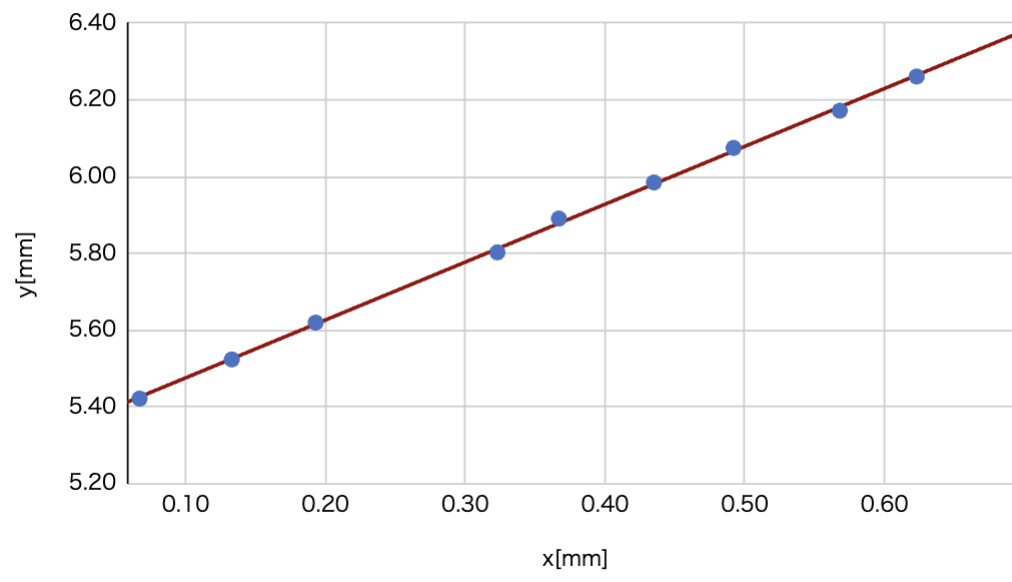
\includegraphics[width=150mm]{actA.png}
  \caption{$x:h_2-h_1とy:h_2の関係$}
  \end{center}
\end{figure}
  

\clearpage


\subsection[short]{サファイア基盤}


\begin{table}[H]
  \caption{$h_0,h_1,h_2$の測定値}
  \label{table:SpeedOfLight}
  \centering
  \begin{tabular}{|c||r|r|r|r|r|r|r|r|r|r|}
    \hline
    番号 & $h_0$ & $h_1$ & x & y & x*x & x*y & y' & v & $v^2\times10^8$\\
    &[mm] & [mm] & $h_2-h_1$[mm] & $h_2$[mm] & [$mm^2$] & [$mm^2$] & [mm] & [mm] & [$mm^2$]\\
    \hline \hline
    1 & 5.33 & 5.35 & 0.04 & 5.39 & 0.0017 & 0.2210 & 5.391837839 & -0.0008 & 64 \\
    2 & 5.33 & 5.35 & 0.07 & 5.43 & 0.0053 & 0.3960 & 5.446345125 & -0.0213 & 45369 \\
    3 & 5.33 & 5.40 & 0.08 & 5.48 & 0.0067 & 0.4497 & 5.461675299 & 0.0223 & 49729 \\
    4 & 5.33 & 5.41 & 0.12 & 5.53 & 0.0154 & 0.6860 & 5.533216112 & -0.0012 & 144 \\
    5 & 5.33 & 5.43 & 0.15 & 5.58 & 0.0240 & 0.8655 & 5.586020045 & -0.0020 & 400 \\
    6 & 5.33 & 5.45 & 0.19 & 5.64 & 0.0357 & 1.0661 & 5.643934036 & -0.0029 & 841 \\
    7 & 5.33 & 5.47 & 0.22 & 5.69 & 0.0462 & 1.2227 & 5.827896126 & -0.1409 & 1985281 \\
    8 & 5.33 & 5.50 & 0.24 & 5.74 & 0.0566 & 1.3656 & 6.6218791 & -0.8839 & 78127921 \\
    9 & 5.33 & 5.52 & 0.27 & 5.79 & 0.0724 & 1.5575 & 5.780202251 & 0.0098 & 9604 \\
    10 & 5.33 & 5.53 & 0.31 & 5.84 & 0.0980 & 1.8285 & 5.855149769 & -0.0131 & 17161 \\
    \hline
    sum &  &  & 1.70 & 56.11 & 0.3621 & 9.6588 &  & 0.0000 & 80236514 \\
    \hline
  \end{tabular}


\end{table}

実験結果をプロットした結果,1回目と3回目の測定結果が明らかに外れ値であったため,除外して計算を行う.修正した結果の表は以下の通り.

\begin{table}[H]
  \caption{$h_0,h_1,h_2$の測定値(外れ値修正後)}
  \label{table:SpeedOfLight}
  \centering
  \begin{tabular}{|c||r|r|r|r|r|r|r|r|r|r|}
    \hline
    番号 & $h_0$ & $h_1$ & x & y & x*x & x*y & y' & v & $v^2\times10^8$\\
    &[mm] & [mm] & $h_2-h_1$[mm] & $h_2$[mm] & [$mm^2$] & [$mm^2$] & [mm] & [mm] & [$mm^2$]\\
    \hline \hline
    2 & 5.33 & 5.35 & 0.07 & 5.43 & 0.0053 & 0.3960 & 5.436661651 & -0.0117 & 13599.40949 \\
    4 & 5.33 & 5.41 & 0.12 & 5.53 & 0.0154 & 0.6860 & 5.526410689 & 0.0056 & 3124.039218 \\
    5 & 5.33 & 5.43 & 0.15 & 5.58 & 0.0240 & 0.8655 & 5.580964027 & 0.0030 & 921.7133154 \\
    6 & 5.33 & 5.45 & 0.19 & 5.64 & 0.0357 & 1.0661 & 5.640796719 & 0.0002 & 4.132300472 \\
    7 & 5.33 & 5.47 & 0.22 & 5.69 & 0.0462 & 1.2227 & 5.686551131 & 0.0004 & 20.14830531 \\
    8 & 5.33 & 5.50 & 0.24 & 5.74 & 0.0566 & 1.3656 & 5.727026188 & 0.0110 & 12042.45475 \\
    9 & 5.33 & 5.52 & 0.27 & 5.79 & 0.0724 & 1.5575 & 5.781579525 & 0.0084 & 7090.43916 \\
    10 & 5.33 & 5.53 & 0.31 & 5.84 & 0.0980 & 1.8285 & 5.859010069 & -0.0170 & 28934.24401 \\

   \hline
   sum &  &  & 1.58 & 45.24 & 0.3537 & 8.9881 &  & 0.0000 & 65736.58055 \\
    \hline
  \end{tabular}


\end{table}


\clearpage


理論(5),(6)より,\\

$a=\dfrac{8\times8.9811-1.58\times45.24}{8\times0.3537-1.58^2}=1.759785076$\\

$b=\dfrac{0.3537\times45.24-1.58\times8.9811}{8\times0.3537-1.58^2}=5.30819734$\\

理論(8)(9)より,\\

$E_a=\pm0.6745\sqrt{\dfrac{8}{8\times0.3537-1.58^2}\times\dfrac{65736.58055\times10^{-8}}{6}}=0.0339764987$\\

$E_b=\pm0.6745\sqrt{\dfrac{0.3537}{8\times0.3537-1.58^2}\dfrac{65736.58055\times10^{-8}}{6}}=0.007143654802$\\

したがって,\\

$a=1.759785076\pm0.0339764987=1.760\pm0.034$\\

$b=5.30819734\pm0.007143654802=5.308\pm0.007$\\

したがって,サファイア基板の屈折率は\\

$u=a=1.760\pm0.034$\\

また,\\

$h_0=b=5.308\pm0.007$\\


\begin{figure}[h]
  \begin{center}
  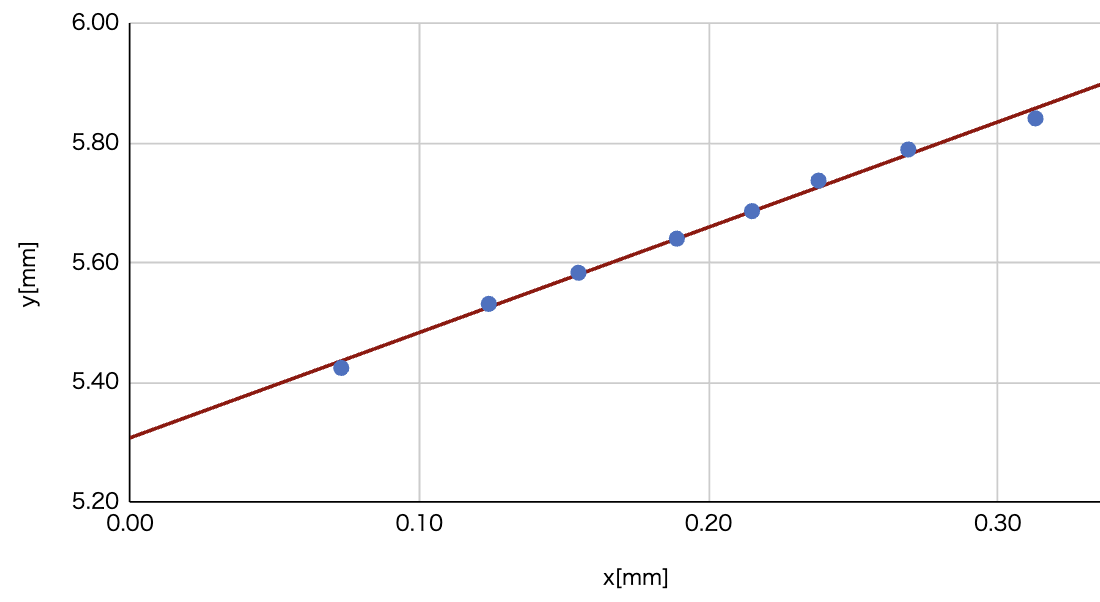
\includegraphics[width=150mm]{actB.png}
  \caption{$x:h_2-h_1とy:h_2の関係$}
  \end{center}
\end{figure}

\clearpage

\blue{2回目が測定ミスであったため,2回目のみを除外して計算を行った.修正後の表は以下の通り}\\

\begin{table}[H]
  \caption{$h_0,h_1,h_2$の測定値(外れ値修正後)}
  \label{table:SpeedOfLight}
  \centering
  \begin{tabular}{|c||r|r|r|r|r|r|r|r|r|r|}
    \hline
    番号 & $h_0$ & $h_1$ & x & y & x*x & x*y & y' & v & $v^2\times10^8$\\
    &[mm] & [mm] & $h_2-h_1$[mm] & $h_2$[mm] & [$mm^2$] & [$mm^2$] & [mm] & [mm] & [$mm^2$]\\
    \hline \hline
    1 & 5.33 & 5.35 & 0.04 & 5.39 & 0.0016 & 0.2156 & 5.397753401 & -0.0078 & 6011.522824 \\
    3 & 5.33 & 5.40 & 0.08 & 5.48 & 0.0064 & 0.4384 & 5.464395345 & 0.0156 & 24350.52469 \\
    4 & 5.33 & 5.41 & 0.12 & 5.53 & 0.0154 & 0.6860 & 5.537701484 & -0.0057 & 3250.692028 \\
    5 & 5.33 & 5.43 & 0.15 & 5.58 & 0.0240 & 0.8655 & 5.589348991 & -0.0053 & 2861.170313 \\
    6 & 5.33 & 5.45 & 0.19 & 5.64 & 0.0357 & 1.0661 & 5.645994643 & -0.0050 & 2494.64635 \\
    7 & 5.33 & 5.47 & 0.22 & 5.69 & 0.0462 & 1.2227 & 5.689311907 & -0.0023 & 534.4915161 \\
    8 & 5.33 & 5.50 & 0.24 & 5.74 & 0.0566 & 1.3656 & 5.727631025 & 0.0104 & 10751.56382 \\
    9 & 5.33 & 5.52 & 0.27 & 5.79 & 0.0724 & 1.5575 & 5.779278532 & 0.0107 & 11494.98756 \\
    10 & 5.33 & 5.53 & 0.31 & 5.84 & 0.0980 & 1.8285 & 5.852584671 & -0.0106 & 11203.52542 \\

   \hline
   sum &  &  & 1.62 & 50.68 & 0.3563 & 9.2460 &  & 0.0000 & 72953.12452 \\
    \hline
  \end{tabular}


\end{table}

\blue{理論(5),(6)より,}\\

\blue{$a=\dfrac{9\times9.2460-1.62\times50.68}{9\times0.3563-1.62^2}=1.666048607$}\\

\blue{$b=\dfrac{0.3563\times50.68-1.62\times9.2460}{9\times0.3563-1.62^2}=5.331111457$}\\

\blue{理論(8)(9)より,}\\

\blue{$E_a=\pm0.6745\sqrt{\dfrac{9}{9\times0.3563-1.62^2}\times\dfrac{72953.12452\times10^{-8}}{7}}=0.02729542099$}\\

\blue{$E_b=\pm0.6745\sqrt{\dfrac{0.3563}{9\times0.3563-1.62^2}\dfrac{72953.12452\times10^{-8}}{7}}=0.005431118162$}\\

\blue{したがって,}\\

\blue{$a=1.666048607\pm0.02729542099=1.666\pm0.027$}\\

\blue{$b=5.331111457\pm0.005431118162=5.331\pm0.005$}\\

\blue{したがって,サファイア基板の屈折率は}\\

\blue{$u=a=1.666\pm0.027$}\\

\blue{また,}\\

\blue{$h_0=b=5.331\pm0.005$}\\

\begin{figure}[h]
  \begin{center}
  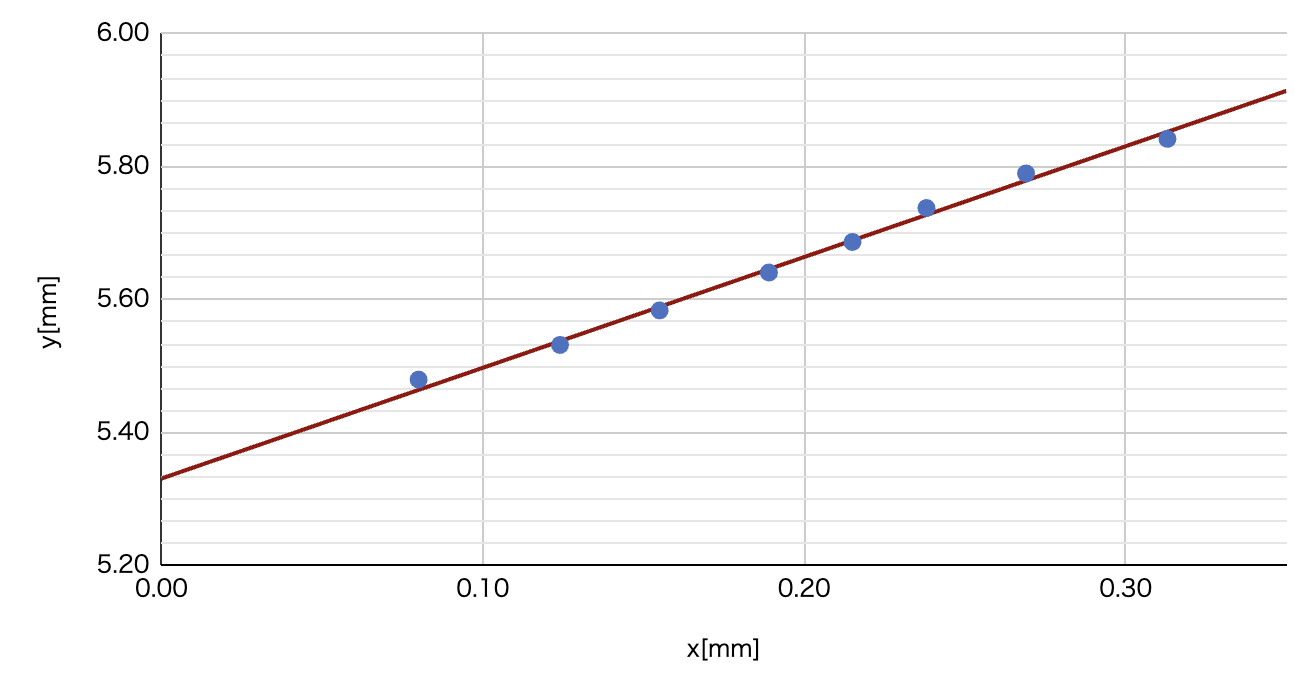
\includegraphics[width=150mm]{actD.png}
  \caption{$x:h_2-h_1とy:h_2の関係(修正版)$}
  \end{center}
\end{figure}


\clearpage

\subsection[short]{水}


\begin{table}[H]
  \caption{$h_0,h_1,h_2$の測定値}
  \label{table:SpeedOfLight}
  \centering
  \begin{tabular}{|c||r|r|r|r|r|r|r|r|r|r|}
    \hline
    番号 & $h_0$ & $h_1$ & x & y & x*x & x*y & y' & v & $v^2\times10^8$\\
    &[mm] & [mm] & $h_2-h_1$[mm] & $h_2$[mm] & [$mm^2$] & [$mm^2$] & [mm] & [mm] & [$mm^2$]\\
    \hline \hline
    1 & 53.70 & 54.24 & 1.15 & 55.39 & 1.3225 & 63.6985 & 55.4687 & -0.0787 & 618907.0297 \\
    2 & 53.70 & 55.67 & 4.96 & 60.63 & 24.6016 & 300.7248 & 60.5279 & 0.1021 & 1042440.49 \\
    3 & 53.70 & 56.48 & 7.62 & 64.10 & 58.0644 & 488.4420 & 64.0601 & 0.0399 & 159477.0738 \\
    4 & 53.70 & 57.41 & 10.73 & 68.14 & 115.1329 & 731.1422 & 68.1898 & -0.0498 & 247780.8545 \\
    5 & 53.70 & 58.42 & 13.70 & 72.12 & 187.6900 & 988.0440 & 72.1336 & -0.0136 & 18458.81048 \\
    \hline
    sum &  &  & 38.16 & 320.38 & 386.8114 & 2572.0515 &  & 0.0000 & 2087064.258 \\
    \hline
  \end{tabular}


\end{table}

理論(5),(6)より,\\

$a=\dfrac{5\times2572.0515-38.16\times320.38}{5\times386.8114-38.16^2}=1.327881727$\\

$b=\dfrac{386.8114\times320.38-38.16\times2572.0515}{5\times386.8114-38.16^2}=53.94160666$\\

理論(8)(9)より,\\

$E_a=\pm0.6745\sqrt{\dfrac{5}{5\times386.8114-38.16^2}\times\dfrac{2087064.258\times10^{-8}}{3}}=0.00575464741$\\

$E_b=\pm0.6745\sqrt{\dfrac{386.8114}{5\times386.8114-38.16^2}\dfrac{2087064.258\times10^{-8}}{3}}=0.05061547885$\\

したがって,\\

$a=1.327881727\pm0.00575464741=1.328\pm0.006$\\

$b=53.94160666\pm0.05061547885=53.94\pm0.051$\\

したがって,水の屈折率は\\

$u=a=1.328\pm0.006$\\

また,\\

$h_0=b=53.94\pm0.051$\\

\begin{figure}[h]
  \begin{center}
  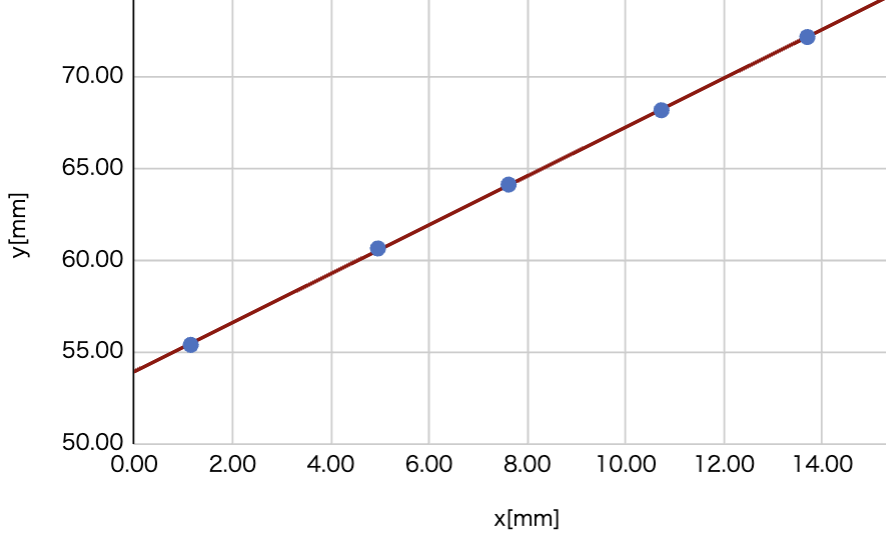
\includegraphics[width=150mm]{actC.png}
  \caption{$x:h_2-h_1とy:h_2の関係$}
  \end{center}
\end{figure}

\clearpage

 
 
\section{考察}

 参考文献[1][2]より,クラウンガラス,サファイア,水の屈折率はそれぞれ,1.47〜1.69,1.760,1.33であり,3つの実験結果から得られた値は全て,理論値と誤差の範囲で一致していた.\\
 
 そのため,実験は概ねうまく行うことができたと思われるが,ガラス基板,サファイア基板の測定については,測定値のプロットの段階で見つかった明らかな外れ値については排除して計算しているため,水の屈折率の結果と比べ,確率誤差が大きくなっている.\\

 大きな外れ値が出た理由として,「ピントがあった」と思う範囲が感覚的に広く,顕微鏡を除く役割の交代や,計測の疲れなどが誤差を生み出してしまっていると考えられる.\\

 \blue{参考文献[1][2]より,クラウンガラス,サファイア,水の屈折率はそれぞれ,1.47〜1.69(λ=589.3[nm]),1.760(λ=590[nm]),1.33(λ=589.3[nm])であり,サファイアのみ実験値と公称値の間に誤差が生じた(-3.81〜6.88\%).}\\

 \blue{誤差の原因として,「ピントがあった」と思う範囲の曖昧さや計測の疲れなどの人為的な面が大きいと考えられる.}





\end{document}
